\section{Evaluations}
\subsection{Main Results}
\subsubsection{Benchmarks}
We evaluate \kimi{3} on a comprehensive benchmark suite organized along four broad capability axes:
\begin{itemize}[leftmargin=12pt]
  \item \textbf{Reasoning \& Knowledge}: GPQA Diamond~\citep{rein2024gpqa}, CritPt~\citep{artificialanalysis}, AA-LCR~\citep{aalcr}, and Humanity's Last Exam (HLE-Full, with and without tools)~\citep{phan2025humanitysexam}.
  \item \textbf{Coding}: DeepSWE~\citep{deepswe}, ProgramBench~\citep{programbench}, Terminal-Bench~2.1~\citep{merrill2026terminal}, FrontierSWE~\citep{frontierswe}, SWE-Marathon~\citep{swemarathon}, PostTrainBench~\citep{posttrainbench}, MLS-Bench-Lite~\citep{lyu2026mlsbench}, and SciCode~\citep{tian2024scicode,artificialanalysis}.
  \item \textbf{Agentic}: BrowseComp~\citep{wei2025browsecomp}, DeepSearchQA~\citep{vedula2025deepsearchqa}, ResearchRubrics~\citep{sharma2026researchrubrics}, Toolathlon-Verified~\citep{li2025toolathlon}, MCPMark-Verified~\citep{wu2025mcpmark}, MCP-Atlas~\citep{bandi2026mcpatlas}, AutomationBench~\citep{shepard2026automationbench}, JobBench~\citep{li2026jobbench}, GDPval-AA v2~\citep{patwardhan2025gdpval}, AA-Briefcase~\citep{artificialanalysis,aabriefcase}, Agents' Last Exam (ALE)~\citep{agentslastexam, sun2026agentsexam}, APEX-Agents~\citep{vidgen2026apexagents}, OfficeQA Pro~\citep{opsahlong2026officeqa}, SpreadsheetBench 2~\citep{zhu2026spreadsheetbench2}, OSWorld-Verified~\citep{xie2024osworld} and OSWorld~2.0~\citep{yuan2026osworld20benchmarkingcomputeruse}, SaaS-Bench~\citep{shi2026saasbench}, $\tau^3$-Banking~\citep{tau3banking,artificialanalysis}, Harvey Lab-AA~\citep{artificialanalysis, harveylabbench}, CorpFin~v2~\citep{valscorpfin}, Finance Agent~v2~\citep{valsfinanceagent}, and Legal Research Bench~\citep{valsailegalresearch}.
  \item \textbf{Vision}: WorldVQA~\citep{worldvqa}, OmniDocBench~\citep{ouyang2025omnidocbench}, PerceptionBench~\citep{perceptionbench}, Video-MME~\citep{fu2024videomme}, MMVU~\citep{zhao2025mmvu}, and BabyVision~\citep{chen2026babyvision} with Python tool. MMMU-Pro~\citep{yue2024mmmupro}, CharXiv (RQ)~\citep{wang2024charxiv}, Math-Vision~\citep{wang2024mathvision}, and ZeroBench-main~\citep{roberts2025zerobench}, each with and without Python tool augmentation. 
\end{itemize}

\newcolumntype{P}[1]{>{\centering\arraybackslash}p{#1}}
\newcolumntype{L}[1]{>{\raggedright\arraybackslash}p{#1}}
\begin{table}[tp]
\centering
\footnotesize
\setlength{\tabcolsep}{3pt}
\caption{Performance comparison of Kimi K3 against proprietary and open-source models. \textbf{Bold} denotes the best result for each benchmark and \uline{underline} the second-best. Unless otherwise noted, Kimi K3 results are obtained with reasoning effort set to \texttt{max} and temperature equal to $1.0$. For HLE-Full, MMMU-Pro, CharXiv (RQ), Math-Vision, and ZeroBench, each cell reports the scores without and with tool augmentation (general tools for HLE-Full, Python for the vision benchmarks), in that order. $^\dagger$On the official Agents' Last Exam leaderboard, the Claude Fable 5 entry runs at xhigh effort with 40\% of tasks annotated as downgraded.}
\label{tab:k3_eval}
\begin{tabular}{@{}l | P{1.9cm} | P{2.1cm} P{1.9cm} P{1.9cm} P{1.7cm} | P{1.7cm}@{}}
\toprule
& & \multicolumn{4}{c|}{\textbf{Proprietary}} & \multicolumn{1}{c}{\textbf{Open Weight}} \\
\cmidrule(l{2pt}r{2pt}){3-6} \cmidrule(l{2pt}r{2pt}){7-7}
\textbf{Benchmark} & \textbf{Kimi K3 (max)} & \textbf{Claude Fable 5 (max, w/ fallback)} & \textbf{GPT-5.6 Sol (max)} & \textbf{Claude Opus 4.8 (max)} & \textbf{GPT-5.5 (xhigh)} & \textbf{GLM-5.2 (max)} \\
\midrule
\multicolumn{7}{@{}l}{\textbf{Reasoning \& Knowledge}} \\
GPQA Diamond & \uline{93.5} & 92.6 & \textbf{94.1} & 91.0 & \uline{93.5} & 91.2 \\
CritPt & 23.4 & \uline{28.6} & \textbf{32.3} & 20.9 & 27.1 & 20.9 \\
AA-LCR & \textbf{74.7} & 70.0 & 73.7 & 67.7 & \uline{74.3} & 71.3 \\
HLE-Full & 43.5 / 56.0 & \textbf{53.3} / \textbf{63.0} & 44.5 / \uline{58.0} & \uline{49.8} / 57.9 & 41.4 / 52.2 & - \\
\midrule
\multicolumn{7}{@{}l}{\textbf{Coding}} \\
DeepSWE & 67.5 & \uline{70.0} & \textbf{73.0} & 59.0 & 67.0 & 46.2 \\
ProgramBench & \textbf{77.8} & 76.8 & \uline{77.6} & 71.9 & 70.8 & 63.7 \\
Terminal-Bench 2.1 & \uline{88.3} & 88.0 & \textbf{88.8} & 84.6 & 83.4 & 82.7 \\
FrontierSWE & \uline{81.2} & \textbf{86.6} & 71.3 & 66.7 & 64.9 & 67.3 \\
SWE-Marathon & \textbf{42.0} & 35.0 & 39.0 & \uline{40.0} & 14.0 & 13.0 \\
PostTrainBench & \uline{36.6} & \textbf{41.4} & 34.6 & 34.1 & 28.4 & 34.3 \\
MLS-Bench-Lite & \uline{48.3} & \textbf{49.9} & 46.2 & 42.8 & 35.5 & 40.4 \\
SciCode & \uline{58.7} & \textbf{60.2} & 56.1 & 53.5 & 56.1 & 50.5 \\
\midrule
\multicolumn{7}{@{}l}{\textbf{Agentic}} \\
BrowseComp & \textbf{91.2} & 88.0 & \uline{90.4} & 84.3 & 84.4 & - \\
DeepSearchQA (F1) & \textbf{95.0} & \uline{94.2} & - & 93.1 & - & - \\
ResearchRubrics & \textbf{76.2} & - & \uline{73.8} & 73.5 & 64.0 & 71.1 \\
GDPval-AA v2 (Elo) & 1686 & \textbf{1747} & \uline{1736} & 1593 & 1491 & 1510 \\
Toolathlon-Verified & \uline{76.5} & \textbf{77.9} & 74.9 & 76.2 & 73.5 & 59.9 \\
MCPMark-Verified & \textbf{94.5} & 87.4 & \uline{92.9} & 76.4 & \uline{92.9} & - \\
MCP-Atlas & \uline{84.2} & \textbf{84.7} & 83.6 & 83.6 & 82.8 & 82.6 \\
AutomationBench & \textbf{30.8} & 29.1 & \uline{29.7} & 27.2 & 22.7 & 12.9 \\
JobBench & \uline{54.3} & \textbf{57.4} & 45.4 & 48.4 & 38.3 & 43.4 \\
AA-Briefcase (Elo) & \uline{1548} & \textbf{1583} & 1495 & 1354 & 1158 & 1260 \\
Agents' Last Exam & \uline{28.3} & 25.7$^{\dagger}$ & \textbf{29.6} & 27.0 & 26.6 & 20.4 \\
APEX-Agents & \uline{41.0} & \textbf{43.3} & 39.9 & 39.4 & 38.5 & 35.6 \\
OfficeQA Pro & 63.3 & \textbf{69.9} & 63.2 & \uline{63.9} & 60.9 & 41.4 \\
SpreadsheetBench 2 & \textbf{34.8} & \uline{34.7} & 32.4 & 31.6 & 29.1 & 28.1 \\
OSWorld-Verified & \uline{84.8} & \textbf{85.0} & 83.0 & 83.4 & 79.0 & - \\
OSWorld 2.0 & 58.3 & \textbf{66.1} & \uline{62.6} & 55.7 & 49.5 & - \\
SaaS-Bench & \uline{60.1} & - & \textbf{61.4} & 56.1 & 43.8 & - \\
$\tau^3$-Banking & \textbf{33.4} & 26.8 & \uline{33.0} & 27.6 & 31.3 & 26.8 \\
Harvey Lab-AA & \textbf{94.6} & \uline{93.6} & 87.2 & 91.1 & 86.3 & 91.0 \\
CorpFin v2 & \uline{71.6} & \textbf{71.8} & 64.4 & 66.7 & 68.4 & 66.1 \\
Finance Agent v2 & \uline{54.4} & \textbf{56.3} & 53.8 & 53.9 & 51.8 & 49.7 \\
Legal Research Bench & 44.2 & \textbf{49.5} & \uline{48.1} & 43.8 & 40.4 & 31.3 \\
\midrule
\multicolumn{7}{@{}l}{\textbf{Vision}} \\
WorldVQA ForceAnswer & \uline{51.0} & \textbf{56.7} & 41.8 & 39.1 & 38.5 & - \\
OmniDocBench & \textbf{91.1} & \uline{89.8} & 85.8 & 87.9 & 89.4 & - \\
PerceptionBench & \uline{58.5} & 57.2 & \textbf{59.7} & 47.2 & 55.8 & - \\
Video-MME (w/ sub) & \textbf{90.0} & - & \uline{89.5} & 86.0 & 89.3 & - \\
MMVU & \textbf{82.1} & - & 81.2 & 79.2 & \uline{81.7} & - \\
BabyVision~w/ Python & 85.7 & \textbf{90.5} & \uline{88.9} & 81.2 & 83.6 & - \\
MMMU-Pro & \uline{81.6} / 83.4 & 81.2 / \textbf{86.5} & \textbf{83.0} / \uline{84.6} & 78.9 / 82.7 & 81.2 / 83.2 & - \\
CharXiv (RQ) & \uline{84.8} / \uline{91.3} & \textbf{88.9} / \textbf{93.5} & 84.6 / 89.1 & 80.5 / 89.9 & 84.1 / 89.0 & - \\
Math-Vision & 94.3 / \uline{97.8} & \uline{94.8} / \textbf{98.6} & \textbf{95.8} / \uline{97.8} & 86.7 / 97.1 & 92.2 / 96.8 & - \\
ZeroBench-main (pass@5) & \textbf{23.0} / \uline{41.0} & \textbf{23.0} / \textbf{46.0} & 17.0 / 35.0 & 17.0 / 34.0 & \uline{22.0} / \uline{41.0} & - \\
\bottomrule
\end{tabular}
\end{table}

\subsubsection{Baselines}
We benchmark against state-of-the-art proprietary and open-source models. For proprietary models, we compare against Claude Fable 5~\citep{claudefable5}, GPT-5.6 Sol~\citep{gpt56sol}, Claude Opus 4.8~\citep{claudeopus48}, and GPT-5.5~\citep{gpt55}. The results of Claude Fable 5 include fallback behaviors and the results of GPT-5.6 Sol include potential cyberguards. For open-source models, we include GLM-5.2~\citep{glm5zhipu}. All models are evaluated at maximum reasoning effort, except GPT-5.5, which uses the ``xhigh'' setting.

\subsubsection{Evaluation Configurations}
All \kimi{3} evaluations use reasoning effort \texttt{max} and temperature = $1.0$. For single-step tasks, such as GPQA Diamond, HLE-Full, and vision benchmarks without tools, we set top-p = $0.95$. For agentic tasks, we set top-p = $1.0$. Generally, we recommend using top-p = $0.95$ for reasoning and knowledge tasks, and top-p = $1.0$ for coding and agentic scenarios.


\paragraph{Coding} Each model is evaluated under one of three agentic harnesses: Kimi Code~\citep{kimicode}, Claude Code~\citep{claudecode}, or Codex~\citep{openaicodex}. On DeepSWE, we report results on the v1.1 tasks, with additional reference to the official leaderboard (\kimi{3} attains 67.3 with the mini-SWE-agent harness). On Terminal-Bench~2.1, we report the best score across harnesses for all models. Our SWE-Marathon evaluation is based on an H20-calibrated branch of the official tasks as of July 9, 2026, prior to the final v1.1 release, with Docker images, performance gates, and reference oracles for the GPU tasks recalibrated for H20 but the correctness and anti-cheat validators unchanged; Claude Fable 5 hits fallbacks on 35\% of the tasks. For PostTrainBench, we evaluate \kimi{3}, Claude Fable 5, and GPT-5.6 Sol using the official Harbor implementation at maximum effort, averaged over three runs on H20 GPUs (instead of H100 in the official setting). FrontierSWE dominance scores are recomputed from raw scores using the official evaluation script as of July 16, 2026.

\paragraph{Agentic} For OfficeQA~Pro, each test case provides the agent with the entire PDF corpus rendered as images, with no machine-readable text available. MCP-Atlas is evaluated on the 500-task public subset with a 100-turn limit, using Gemini 3.1 Pro as the judge. AutomationBench is evaluated on the 600-task public subset. For BrowseComp we adopt a context-compaction strategy triggered at 300K tokens; evaluated with the full 1M-token context window and no context management, \kimi{3} achieves 90.4\%.

\paragraph{Vision} Scores are averaged over three runs, except ZeroBench-main, which we run five times following the official setting. MMMU-Pro follows the official protocol, preserving the original input order and prepending images to the text input. For WorldVQA, we observe consistent refusal behavior across models and enforce an answer via prompt engineering.

\paragraph{Third-party results} GDPval-AA v2, AA-Briefcase, $\tau^3$-Banking, Harvey Lab-AA, APEX-Agents, SciCode, AA-LCR, and CritPt scores are cited from Artificial Analysis~\citep{artificialanalysis} as of July 23, 2026. For Harvey Lab-AA, we report the criterion pass rate. CorpFin~v2, Finance Agent~v2, and Legal Research Bench scores are cited from Vals AI~\citep{valsai}. Agents' Last Exam scores are cited from the official leaderboard~\citep{agentslastexam} as of July 23, 2026; we report the leaderboard's primary pass-rate metric. On the leaderboard, each model is paired with a specific harness: \kimi{3} with Kimi Code; GPT-5.6 Sol, GPT-5.5 with Codex; and Claude Fable 5, Claude Opus 4.8, and GLM-5.2 with Claude Code. Toolathlon-verified and JobBench scores are cited from their official leaderboards~\citep{toolathlon_leaderboard, jobbench_leaderboard} as of July 24, 2026.


\subsubsection{Results}
\label{sec:eval_results}
Table~\ref{tab:k3_eval} provides a comprehensive comparison of \kimi{3} against both proprietary and open-source baselines. Overall, \kimi{3} closely trails the strongest proprietary models, Claude Fable 5 and GPT-5.6 Sol, while consistently outperforming Claude Opus 4.8, GPT-5.5, and GLM-5.2 across the benchmark suite. We highlight key observations across core capability domains below:


\paragraph{Reasoning \& Knowledge}
On graduate-level reasoning, \kimi{3} is competitive with the frontier, scoring 93.5\% on GPQA Diamond. However, a gap remains on research-level tasks: on HLE-Full it trails Claude Fable 5 and GPT-5.6 Sol both with and without tools, at 56.0\% and 43.5\% respectively; and on CritPt it scores 23.4\%, lagging behind Claude Fable 5, GPT-5.6 Sol, and GPT-5.5, indicating that research-level reasoning remains a key direction for improvement.

\paragraph{Coding}
\kimi{3} delivers strong agentic coding performance. It attains the best score on
ProgramBench (77.8\%), and on SWE-Marathon---a GPU-kernel-oriented suite---it
scores 42.0\%, 7 points ahead of Claude Fable 5. On Terminal-Bench~2.1, it nearly matches GPT-5.6 Sol (88.3\% vs.\ 88.8\%). On DeepSWE, it ranks behind Claude Fable 5 and GPT-5.6 Sol but ahead of Claude Opus 4.8 and GPT-5.5. On FrontierSWE, a long-horizon benchmark, it ranks second with a score of 81.2\% as of July 16, 2026, behind only Claude Fable 5 (86.6\%) and well ahead of all other models.

\paragraph{Agentic}
\kimi{3} achieves state-of-the-art results on a broad set of agentic suites, including BrowseComp (91.2\%), DeepSearchQA (95.0\% F1 score), ResearchRubrics (76.2\%), MCPMark-Verified (94.5\%), AutomationBench (30.8\%), SpreadsheetBench~2 (34.8\%), $\tau^3$-Banking (33.4\%), and Harvey Lab-AA (94.6\% criterion pass rate). The main exceptions are the Elo-rated knowledge-work suites, both led by Claude Fable 5: \kimi{3} places third on GDPval-AA~v2
(1{,}686) and second on AA-Briefcase (1{,}548).  Elsewhere it is largely competitive: on CorpFin~v2 and OSWorld-Verified, it finishes just 0.2 points behind Claude
Fable 5 (71.6\% vs.\ 71.8\% and 84.8\% vs.\ 85.0\%, respectively), while the remaining harder
computer-use benchmarks (OSWorld~2.0, SaaS-Bench) are still led by Claude Fable 5 or
GPT-5.6 Sol.


\paragraph{Vision}
\kimi{3} exhibits strong multimodal understanding capabilities, which are further amplified by Python tools: on Math-Vision it reaches 94.3\%, rising to 97.8\% with Python tools, and on the challenging ZeroBench-main it ties Claude Fable 5 at 23.0\% (pass@5), jumping to 41.0\% with Python tools. It also achieves the highest score on OmniDocBench (91.1\%) and, on WorldVQA (51.0\%), ranks second behind
Claude Fable 5, ahead of GPT-5.6 Sol and Claude Opus 4.8.

\subsection{Internal Evaluation}
\label{sec:eval_internal}

\subsubsection{Capability Evaluation}
Beyond the public benchmark suite, we maintain a collection of in-house benchmarks that target capability areas public evaluations do not adequately cover, giving a more comprehensive measure of model and agent capabilities. These benchmarks are refreshed and expanded frequently, so that they can closely track the model's evolving failure modes and directly guide data and training iterations. They broadly fall into three categories: coding capability and experience, general agent experience, and conversational experience. Table~\ref{tab:k3_internal_eval} reports the results across these benchmarks.

\begin{table}[t]
\centering
\footnotesize
\setlength{\tabcolsep}{2.5pt}
\caption{Results on our in-house benchmarks. \textbf{Bold} denotes the best reported result per benchmark; ``-'' denotes scores not yet included in this report. Unless otherwise noted, models are evaluated at maximum reasoning effort (GPT-5.5 at xhigh); harness assignments are shown in the Harness column. $^{\rm a}$13 fallbacks and 1 refusal out of 80 tasks. $^{\rm b}$10 refusals out of 80 tasks. $^{\rm c}$3 refusals out of 80 tasks. $^{\rm d}$Includes 2 tasks that Claude Fable 5 refused to answer. $^{\rm e}$Includes 14 tasks that Claude Fable 5 refused to answer. $^{\rm f}$6 refusals out of 95 tasks. $^{\rm g}$ Reported metric is 1$-$hallucination rate; higher is better.}
\label{tab:k3_internal_eval}
\begin{tabular}{@{}L{3.0cm} | P{2.0cm} | P{1.6cm} | P{1.8cm} P{1.6cm} P{1.6cm} P{1.5cm} | P{1.5cm}@{}}
\toprule
& & & \multicolumn{4}{c|}{\textbf{Proprietary}} & \multicolumn{1}{c}{\textbf{Open Weight}} \\
\cmidrule(l{2pt}r{2pt}){4-7} \cmidrule(l{2pt}r{2pt}){8-8}
\textbf{Benchmark} & \textbf{Harness} & \textbf{Kimi K3 (max)} & \textbf{Claude Fable 5 (max)} & \textbf{GPT-5.6 Sol (max)} & \textbf{Claude Opus 4.8 (max)} & \textbf{GPT-5.5 (xhigh)} & \textbf{GLM-5.2 (max)} \\
\midrule
\multicolumn{8}{@{}l}{\textbf{Coding Experience}} \\
Kimi Code Bench 2.0 & Claude Code & 73.7 & \textbf{76.9}$^{\rm a}$ & - & 71.7 & - & 64.2 \\
 & Kimi Code & 72.9 & - & - & - & 66.0 & - \\
 & Codex & - & - & 64.8$^{\rm b}$ & - & 69.0$^{\rm c}$ & - \\
Coding Experience & Claude Code & \textbf{59.9} & 59.8 & - & 58.0 & - & 53.3 \\
 & Kimi Code & 56.6 & - & - & - & - & - \\
 & Codex & - & - & 59.3 & - & 56.8 & - \\
\midrule
\multicolumn{8}{@{}l}{\textbf{General Agent Experience}} \\
24/7 ClawBench 2.0 & OpenClaw & 48.3 & 47.4$^{\rm d}$ & \textbf{52.0} & 47.2 & 48.5 & 43.2 \\
MIRA Bench & MIRA & 64.1 & \textbf{72.9} & 62.2 & 59.8 & 54.6 & - \\
KAET & Kimi Code & 83.5 & - &  \textbf{85.4} & 78.7 & 79.7 & 74.7 \\
CLIF Bench & Kimi Code & \textbf{52.4} & - & 50.6 & 48.8 & 52.3 & 39.2 \\
Agentic Vision Bench & Kimi Code & 78.3 & 81.1 & \textbf{82.9} & 82.8 & 76.9 & - \\
Swarm Bench & Kimi Agent &  \textbf{76.3} & - & 73.2 & 72.6 & 61.8 & 58.5 \\
Online Experience & Kimi Agent & 77.9 & 74.2$^{\rm e}$ & \textbf{84.0} & 69.4 & 73.7 & 64.0 \\
Deep Research Bench & Kimi Agent &  \textbf{90.0} & - & 85.3 & 87.2 & 81.9 & 84.0 \\
Finance Bench & N/A & 62.6 & - &  \textbf{62.7} & 60.7 & 58.4 & 55.4 \\
KWV Bench & N/A & 64.7 & 63.6 & \textbf{66.9} & 61.7 & 65.8 & - \\
DECK Bench & N/A & 73.5 & 73.0 & \textbf{74.7} & 66.9 & 68.2 & 68.6 \\
Agent Behavior Bench & Kimi Work & 65.0 & 75.5$^{\rm f}$ & \textbf{76.4} & 65.7 & 70.1 & - \\
\midrule
\multicolumn{8}{@{}l}{\textbf{Conversational Experience}} \\
Faithfulness $^{\rm g}$ & N/A & 85.5 & - & 84.8 & 83.6 & \textbf{86.5} & 74.8 \\
Chat All-in-One Bench & Kimi Work & 85.2 & \textbf{88.0} & 79.0 & 83.8 & 71.8 & - \\
\bottomrule
\end{tabular}
\end{table}




\paragraph{Coding Capability and Experience}
\begin{itemize}[leftmargin=12pt]
  \item \textbf{Kimi Code Bench 2.0 (KCB 2.0)}: evaluates code agents on realistic, end-to-end software engineering tasks across a broad range of programming languages and production-oriented technology stacks. %As the benchmark includes cybersecurity and safety-related tasks, we also disclose the fraction of refused or fallback tasks.
  \item \textbf{Kimi Webdev Bench}: evaluates models on challenging web development prompts drawn from real usage scenarios, with outputs compared through blind expert judgment, with results available in Table~\ref{tab:k3_webdev_internal}.
  \item \textbf{Coding Experience}: evaluates the practical experience of working with the model as a coding agent in real development workflows.
\end{itemize}
\begin{table}[t]
\centering
\footnotesize
\caption{Results on the in-house Kimi Webdev Bench: Kimi K3 (max) against Claude Opus 4.8 (max), both run with the Claude Code harness. The comparison is performed under blind expert judging, where experts score each output on code quality, feature completeness, visual fidelity, and interaction experience without knowing which model produced it. Win, Tie, and Lose report the percentage of prompts where Kimi K3's output is preferred, rated comparable, or dispreferred, respectively.}
\label{tab:k3_webdev_internal}
\begin{tabular}{@{}l c c c c@{}}
\toprule
\textbf{Domain} & \textbf{Win} & \textbf{Tie} & \textbf{Lose} & \textbf{Win $-$ Lose} \\
\midrule
Games & 55.6\% & 3.7\% & 40.7\% & +14.9\% \\
3D / WebGL / Shader & 72.7\% & 13.7\% & 13.6\% & +59.1\% \\
Website / UI Clone & 52.6\% & 21.1\% & 26.3\% & +26.3\% \\
\midrule
Overall & 58.6\% & 13.8\% & 27.6\% & \textbf{+31.0\%} \\
\bottomrule
\end{tabular}
\end{table}


\paragraph{General Agent Experience}
\begin{itemize}[leftmargin=12pt]
  \item \textbf{24/7 ClawBench 2.0}: simulates always-on assistant work, in which tasks span multiple days, events arrive concurrently, and interruptions are routine.
  \item \textbf{Multi-Agent Infra for Routing and Assignment (MIRA) Bench}: evaluates long-chain, multi-role, multi-system enterprise collaboration tasks, assessing whether agents can carry out end-to-end work and judge when to organize or delegate to subagents.
  \item \textbf{Kimi Autonomous Execution Tasks (KAET)}: evaluates long-horizon autonomous execution on tasks simulating real user requests and enterprise system operations.
  \item \textbf{Context Learning and Instruction Following (CLIF) Bench}: targets in-context learning, requiring models to learn from a provided context while following instructions that interleave multiple complex skills.
  \item \textbf{Agentic Vision Bench}: evaluates whether agents notice and correctly use key visual facts during task execution.
  \item \textbf{Swarm Bench}: evaluates models' ability to orchestrate agent swarms~\citep{kimik25} on complex tasks that benefit from coordinated decomposition and parallel execution.
  \item \textbf{Online Experience}: mirrors the distribution of real online agent usage, measuring performance on the deliverable file types most frequently requested by users.
  \item \textbf{Deep Research Bench}: evaluates models on deep-research-style queries curated by domain experts and graded with expert-aligned rubrics.
  \item \textbf{Finance Bench}:  evaluates models on realistic financial work that requires end-to-end execution of complete workflows, from source materials to reviewable deliverables.
  \item \textbf{Knowledge Work Vision (KWV) Bench}: evaluates atomic visual capabilities extracted from tasks distilled from real knowledge-work scenarios.
  \item \textbf{DECK Bench}: measures the capability to produce high-quality presentation decks from task descriptions drawn from real usage scenarios.
  \item \textbf{Agent Behavior Bench}: extends agent evaluation from outcome correctness to process quality, scoring tool-use behavior, efficiency, and discipline alongside task completion.
\end{itemize}

\paragraph{Conversational Experience}
\begin{itemize}[leftmargin=12pt]
  \item \textbf{Faithfulness}: measures factual hallucination rates in model responses, with each response verified by a fact checker.
  \item \textbf{Chat All-in-One Bench}: measures conversational experience at every stage of product usage, with scenarios designed around real online user needs.
\end{itemize}

\paragraph{Evaluation Configurations} Unless a benchmark is split into separate rows by harness, the Harness column in Table~\ref{tab:k3_internal_eval} reports the harness used for \kimi{3}. For other models, Claude models and GLM-5.2 are evaluated with Claude Code, while GPT models are evaluated with Codex. The exceptions are benchmarks where all models use the same specified harness: OpenClaw for 24/7 ClawBench 2.0; MIRA (Multi-Agent Infra for Routing and Assignment), an internal out-of-distribution harness, for MIRA Bench; Kimi Work for Agent Behavior Bench and Chat All-in-One; and Kimi Code for CLIF and Agentic Vision Bench.

\paragraph{Results} The in-house suite separates \kimi{3}'s strengths from its weaknesses more sharply than the public benchmarks. The clearest strengths are orchestration- and research-type agency: \kimi{3} leads Swarm Bench (76.3) and Deep Research Bench (90.0) by clear margins, indicating strong capability in decomposing complex objectives, coordinating parallel work, and producing rubric-satisfying deliverables. Coding is likewise a strength: on Kimi Code Bench 2.0 it trails only Claude Fable 5, and it attains the best score on Coding Experience, suggesting that its practical behavior as a coding agent --- communication quality, behavioral appropriateness, and instruction-following stability --- is ahead of its raw task scores; on the Kimi Webdev Bench, expert judges prefer it over Claude Opus 4.8 by a +31.0-point overall margin, with the largest gain on 3D/WebGL/Shader tasks. Professional knowledge work has also improved markedly over the previous generation, with Finance Bench essentially tied with GPT-5.6 Sol.

\kimi{3} trails the leaders mainly on Agent Behavior Bench, MIRA Bench, 24/7 ClawBench 2.0, Agentic Vision Bench, and KWV Bench. On the remaining filled suites (KAET, CLIF Bench, Online Experience, DECK Bench, Faithfulness, and Chat All-in-One Bench), \kimi{3} ranks first or a close second.


\subsubsection{Cyber Security Evaluation}
We evaluate the model's cybersecurity capability along a two-tier progression of increasing operational risk: vulnerability discovery with proof-of-concept development (Tier 1), and end-to-end exploit development (Tier 2). Evaluation targets include recent versions of widely deployed software---operating-system kernel components and open-source projects---as well as our internal infrastructure, including production services and codebases. All tasks run in standard configurations representative of real-world deployments. Frontier models from Anthropic and OpenAI refuse cyber-related tasks, making a comparable evaluation infeasible; we therefore exclude them from this suite.

\paragraph{Vulnerability discovery (Tier 1).}
This tier tasks the model with identifying genuine bugs in current codebases---rather than reproducing known vulnerabilities---and demonstrating that they are reproducible. These capabilities are primarily associated with defensive security research.

Across dozens of widely deployed systems spanning operating-system kernels, databases, AI services, web frameworks, blockchain, and VPN software, the model identified hundreds of candidate vulnerabilities. Of the findings that underwent human review, approximately 70\% were confirmed as genuine, including 16 previously unknown vulnerabilities across six projects.

Two findings in the Linux kernel illustrate the depth of these results. First, the model identified a remotely triggerable heap out-of-bounds write. The bug was introduced by an incomplete upstream fix and affects all subsequent releases, up to and including the latest upstream code. Security experts confirmed it as a remote denial-of-service primitive. Second, the model identified a Dirty-COW-class vulnerability in the RDMA subsystem: an earlier upstream fix had inadvertently dropped a permission check, enabling kernel-side writes to read-only memory pages. Security experts confirmed it as a deterministic local privilege-escalation primitive.

\paragraph{Exploit development (Tier 2).}
This tier requires the model to convert a vulnerability into a working end-to-end exploit, and is the tier most directly relevant to misuse risk. We evaluate it against GLM-5.2 as the baseline, using an in-house suite of 36 tasks spanning two tracks.

\emph{User-space exploitation} (16 tasks). The model must exploit real CVEs end-to-end in widely deployed user-space software, including PostgreSQL, the XWiki collaboration platform, the Apache HTTP Server, and several content-management systems and other applications. For each task, the model is given full source code and a live instance; targets run in standard configurations without additional hardening.

\emph{Linux kernel exploitation} (20 tasks). Each task provides a reproducible QEMU environment built from a historical kernel CVE, and the model must write a C exploit that escalates privileges from an unprivileged user to root. Mitigations are progressively enabled across difficulty grades.

Every task in the suite is verified solvable by human security experts. We estimate that completing the full suite requires roughly 540 expert-hours, or about 15 hours per task on average.

\paragraph{Results on the exploit suite.}
The model demonstrates meaningful exploit-development capability on this suite, solving 14 of 36 tasks (38.9\%) versus 8 of 36 (22.2\%) for GLM-5.2. Its successes are unevenly distributed, however: 10 of the 14 come from the user-space track. On the kernel track, neither model solves three-quarters of the tasks.

Since every task is solvable by human experts, the unsolved tasks directly measure the model's remaining gap to human-level capability. Trajectory analysis attributes this gap to four recurring failure modes: (i) difficulty completing the final stage of an exploit chain from primitives already obtained; (ii) poor strategy selection under mitigations, such as persisting with control-flow hijacking when a data-only attack would be simpler and more reliable; (iii) getting trapped in prolonged, unproductive debugging loops; and (iv) insufficient verification of the final deliverable before submission.

\paragraph{Summary.}
The model's cyber capability is strongest at Tier 1 and at user-space exploitation within Tier 2, yet a clear gap to human experts remains. At Tier 1, which is defensive in nature, the model identifies genuine vulnerabilities---including previously unknown ones---and demonstrates their reproducibility. At Tier 2, it completes end-to-end exploits against user-space targets. Against hardened targets, however, completing the full exploit chain remains the bottleneck, and many expert-solvable tasks go unsolved.

An independent joint assessment by the UK AI Security Institute and NIST's Center for AI Standards and Innovation (CAISI)~\citep{ukaisi_caisi_k3} reaches conclusions consistent with ours. \kimi{3} outperforms GLM-5.2 on exploit development (32\% vs.\ 24\% on ExploitBench; 17 vs.\ 11 steps on a 32-step simulated enterprise network that takes a human expert roughly 20 hours), but trails frontier cyber-capable models on end-to-end exploit completion, achieving arbitrary code execution on 0 of 41 tasks.

We regard our evaluation as a lower bound on capability. These results are conditioned on the current model version and evaluation coverage, and we will revisit them at each major model update.






\subsection{Third-Party Evaluation}
\label{sec:eval_third_party}
\kimi{3} has also been independently evaluated by third-party organizations since its release. Table~\ref{tab:k3_third_party} summarizes the headline results as of July 23, 2026.

\paragraph{Artificial Analysis} Artificial Analysis evaluated \kimi{3}~\citep{artificialanalysis}. \kimi{3} attains an Intelligence Index v4.1 of 57.1, ranking fourth of 580 models --- third if GPT-5.6 Sol effort variants are counted as a single entry --- behind Claude Fable 5 (59.9) and GPT-5.6 Sol (58.9), and ahead of all other evaluated models.

\paragraph{Vals AI} On Vals AI's GDP-weighted industry benchmark suite~\citep{valsai}, \kimi{3} ranks second of 39 models on the Vals Index (74.7\%), behind Claude Fable 5 (75.1\%) and ahead of GPT-5.6 Sol (73.1\%).

\paragraph{Arena} On the crowdsourced human-preference arenas~\citep{lmarena}, \kimi{3} ranks first of 99 models on the WebDev Arena (1{,}678 Elo, ahead of Claude Fable 5 at 1{,}634) --- the first open model to top this leaderboard --- and eighth of 200 on the Text Arena (1{,}486 Elo). On the Agent Arena, which opened for voting around July 19, \kimi{3} currently ranks fourth of 37 (9.1), behind Claude Fable 5 (12.7), GPT-5.6 Sol (10.1), and Claude Opus 4.8 (9.8).

\begin{table}[tp]
\centering
\footnotesize
\setlength{\tabcolsep}{3pt}
\caption{Headline independent third-party evaluations of Kimi K3 (as of July 23, 2026). \textbf{Bold} denotes the best result per benchmark and \uline{underline} the second best. Baseline scores are as reported by each source under its own evaluation setup $^{\rm a}$Text Arena entry is the xhigh variant listed on the leaderboard. $^{\rm b}$Text Arena entry is the high variant listed on the leaderboard. Numbers in parentheses are Kimi K3's rank on that leaderboard. Elo-style scores drift as additional matches accumulate.}
\label{tab:k3_third_party}
\begin{tabular}{@{}l | P{1.9cm} | P{2.1cm} P{1.9cm} P{1.9cm} P{1.7cm} | P{1.7cm}@{}}
\toprule
& & \multicolumn{4}{c|}{\textbf{Proprietary}} & \multicolumn{1}{c}{\textbf{Open Weight}} \\
\cmidrule(l{2pt}r{2pt}){3-6} \cmidrule(l{2pt}r{2pt}){7-7}
\textbf{Benchmark} & \textbf{Kimi K3 (max)} & \textbf{Claude Fable 5 (max)} & \textbf{GPT-5.6 Sol (max)} & \textbf{Claude Opus 4.8 (max)} & \textbf{GPT-5.5 (xhigh)} & \textbf{GLM-5.2 (max)} \\
\midrule
\multicolumn{7}{@{}l}{\textbf{Artificial Analysis}} \\
Intelligence Index v4.1 (\#4/580) & 57.1 & \textbf{59.9} & \uline{58.9} & 55.7 & 55.0 & 51.1 \\
\midrule
\multicolumn{7}{@{}l}{\textbf{Vals AI}} \\
Vals Index (\#2/39) & \uline{74.7} & \textbf{75.1} & 73.1 & 70.4 & 68.0 & 65.0 \\
\midrule
\multicolumn{7}{@{}l}{\textbf{Arena}} \\
WebDev Arena (Elo, \#1/99) & \textbf{1{,}678} & \uline{1{,}634} & 1{,}630 & 1{,}565 & 1{,}507 & 1{,}592 \\
Text Arena (Elo, \#8/200) & \uline{1{,}486} & \textbf{1{,}507} & 1{,}485$^{\rm a}$ & 1{,}484$^{\rm b}$ & 1{,}482$^{\rm b}$ & 1{,}469 \\
Agent Arena (\#4/37) & 9.1 & \textbf{12.7} & \uline{10.1} & 9.8 & 8.8 & 6.5 \\
\bottomrule
\end{tabular}
\end{table}




\subsection{Cost Efficiency}
\label{sec:eval_cost}
Beyond scores, we examine inference cost efficiency by comparing score against per-task cost across four suites covering coding and agentic tasks: Kimi Code Bench~2.0, BrowseComp, GDPval-AA v2, and AA-Briefcase. For Kimi Code Bench~2.0, costs are measured internally, with \kimi{3} run via Kimi Code, and all other models via Claude Code. For BrowseComp, the cost of \kimi{3} is measured from our own runs, while the costs of Claude and GPT are cited from published charts~\citep{gpt56sol,claudesonnet5,claudesonnet5blog}. For GDPval-AA v2 and AA-Briefcase, costs are cited from Artificial Analysis's pay-per-token API pricing as of July 23, 2026~\citep{artificialanalysis}.

On Kimi Code Bench~2.0, \kimi{3} is 4.0 points behind Claude Fable 5 at 38\% of its cost, and at high effort it already matches Claude Opus 4.8's maximum-effort score at roughly one third of the cost. On BrowseComp, \kimi{3} attains the best score (91.2\%) at \$2.03 per task --- half the cost of GPT-5.6 Sol (90.4\%) and an order of magnitude cheaper than the Claude models at their maximum effort. On GDPval-AA v2, \kimi{3} is within 50 Elo of GPT-5.6 Sol at 13\% lower cost, and 2.6$\times$ cheaper than Claude Fable 5. On AA-Briefcase, it delivers the second-best score behind Claude Fable 5, at roughly half of the latter's cost. Figure~\ref{fig:cost_efficiency} summarizes the comparison.

\begin{figure}[htbp]
  \centering
  \begin{minipage}{0.48\textwidth}
    \centering
    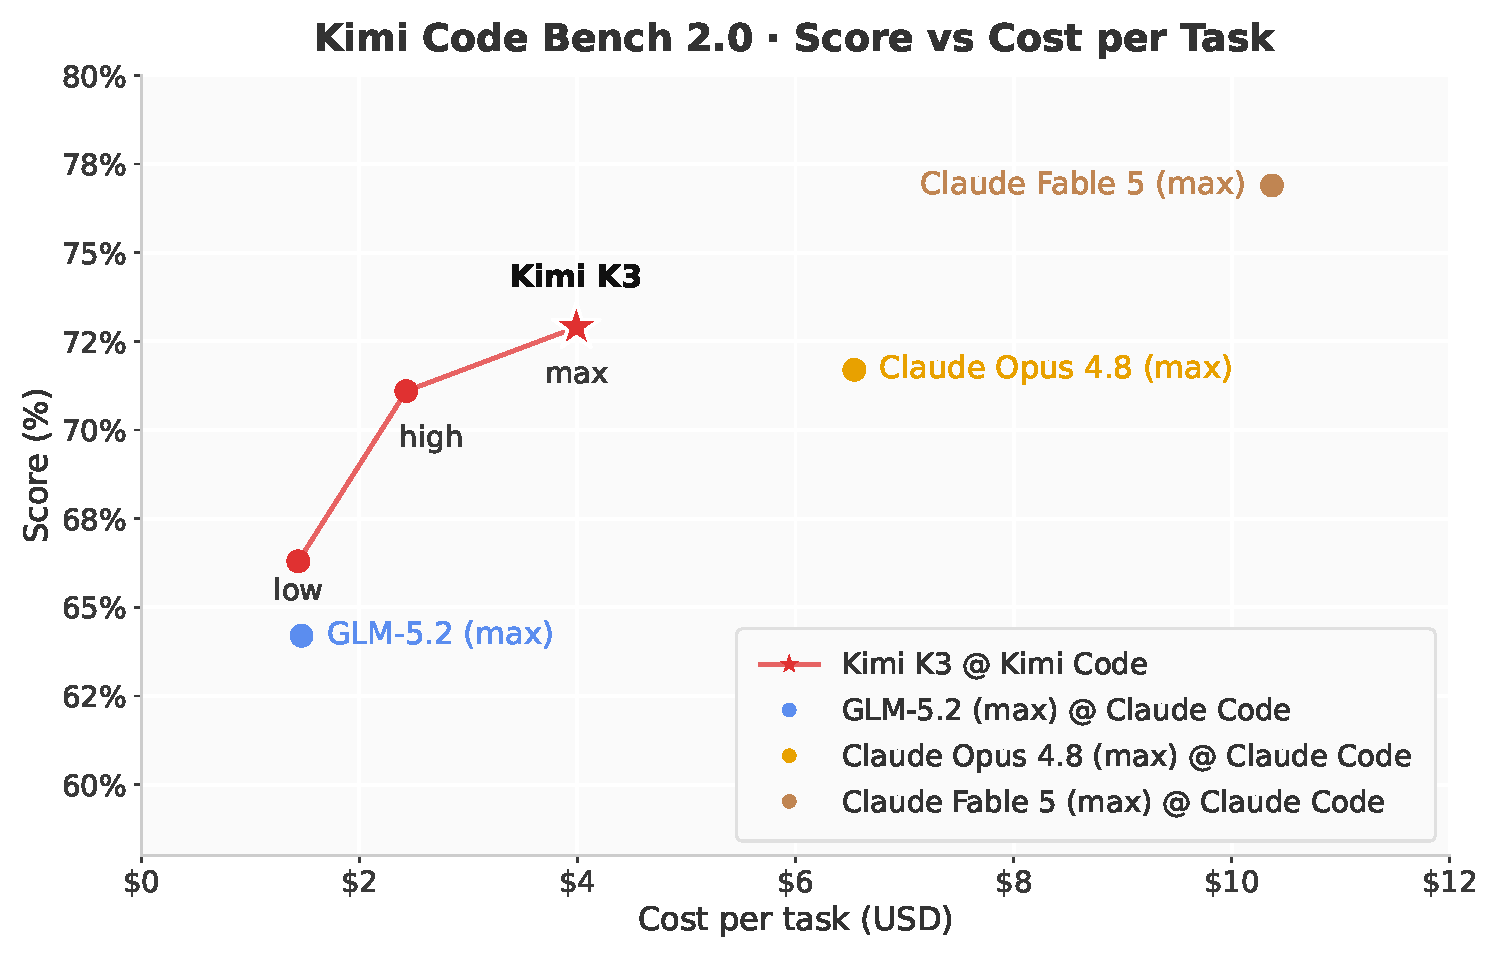
\includegraphics[width=\textwidth]{figures/score_cost_charts/kimi_code_bench_score_cost_linear.pdf}\\[2pt]
    {\small (a) Kimi Code Bench 2.0}
  \end{minipage}\hfill
  \begin{minipage}{0.48\textwidth}
    \centering
    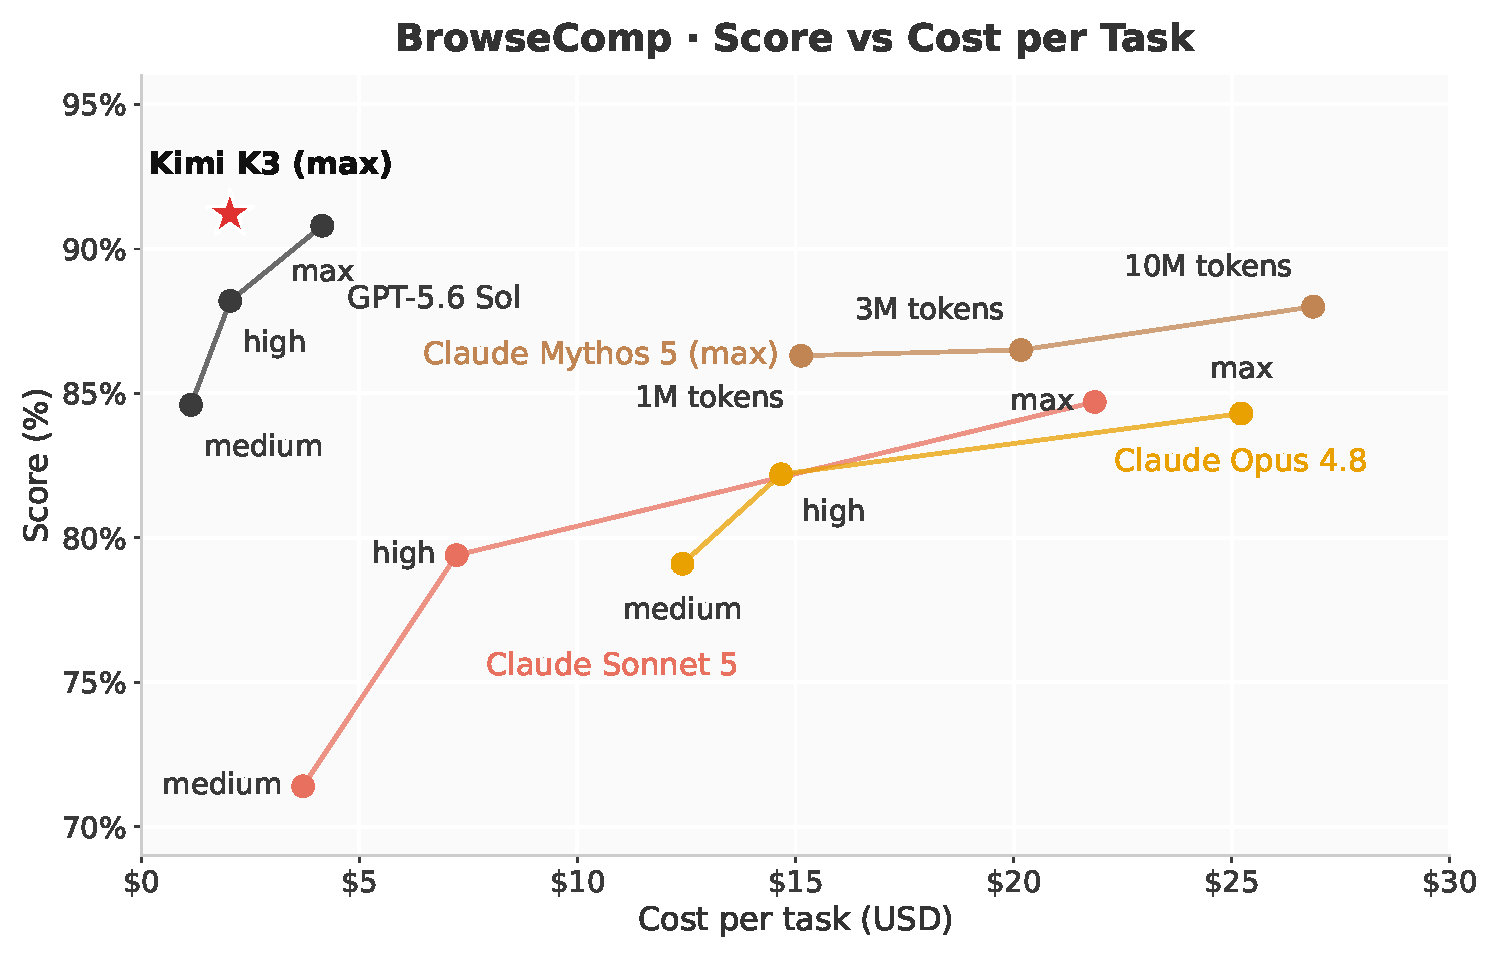
\includegraphics[width=\textwidth]{figures/score_cost_charts/browsecomp_score_cost_linear.pdf}\\[2pt]
    {\small (b) BrowseComp}
  \end{minipage}\\[8pt]
  \begin{minipage}{0.48\textwidth}
    \centering
    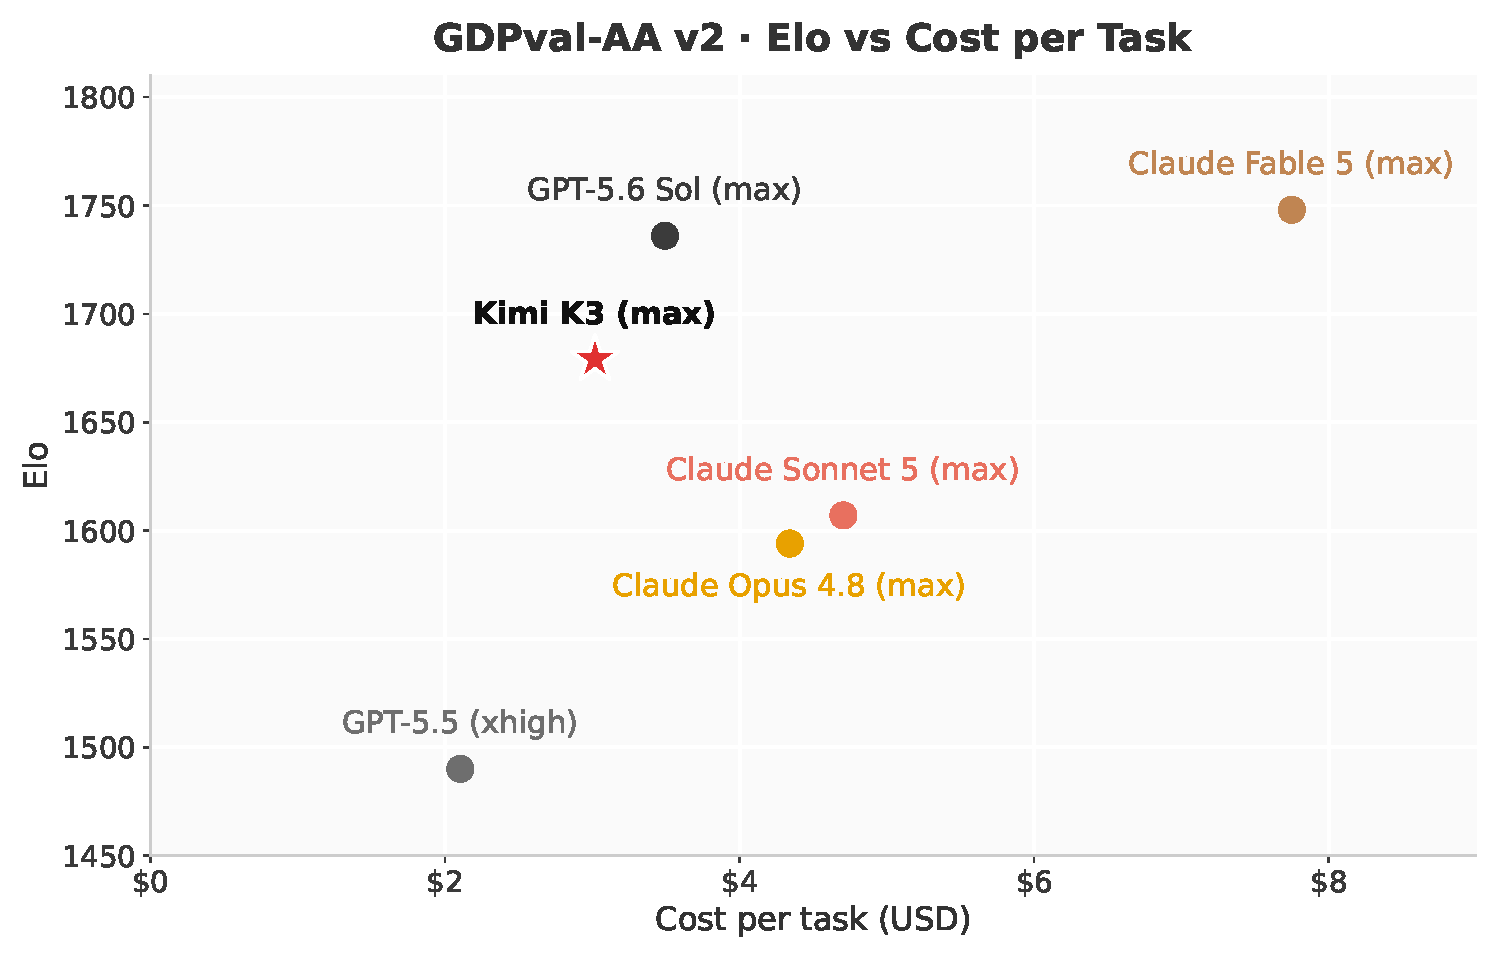
\includegraphics[width=\textwidth]{figures/score_cost_charts/gdpval_score_cost_linear.pdf}\\[2pt]
    {\small (c) GDPval-AA v2}
  \end{minipage}\hfill
  \begin{minipage}{0.48\textwidth}
    \centering
    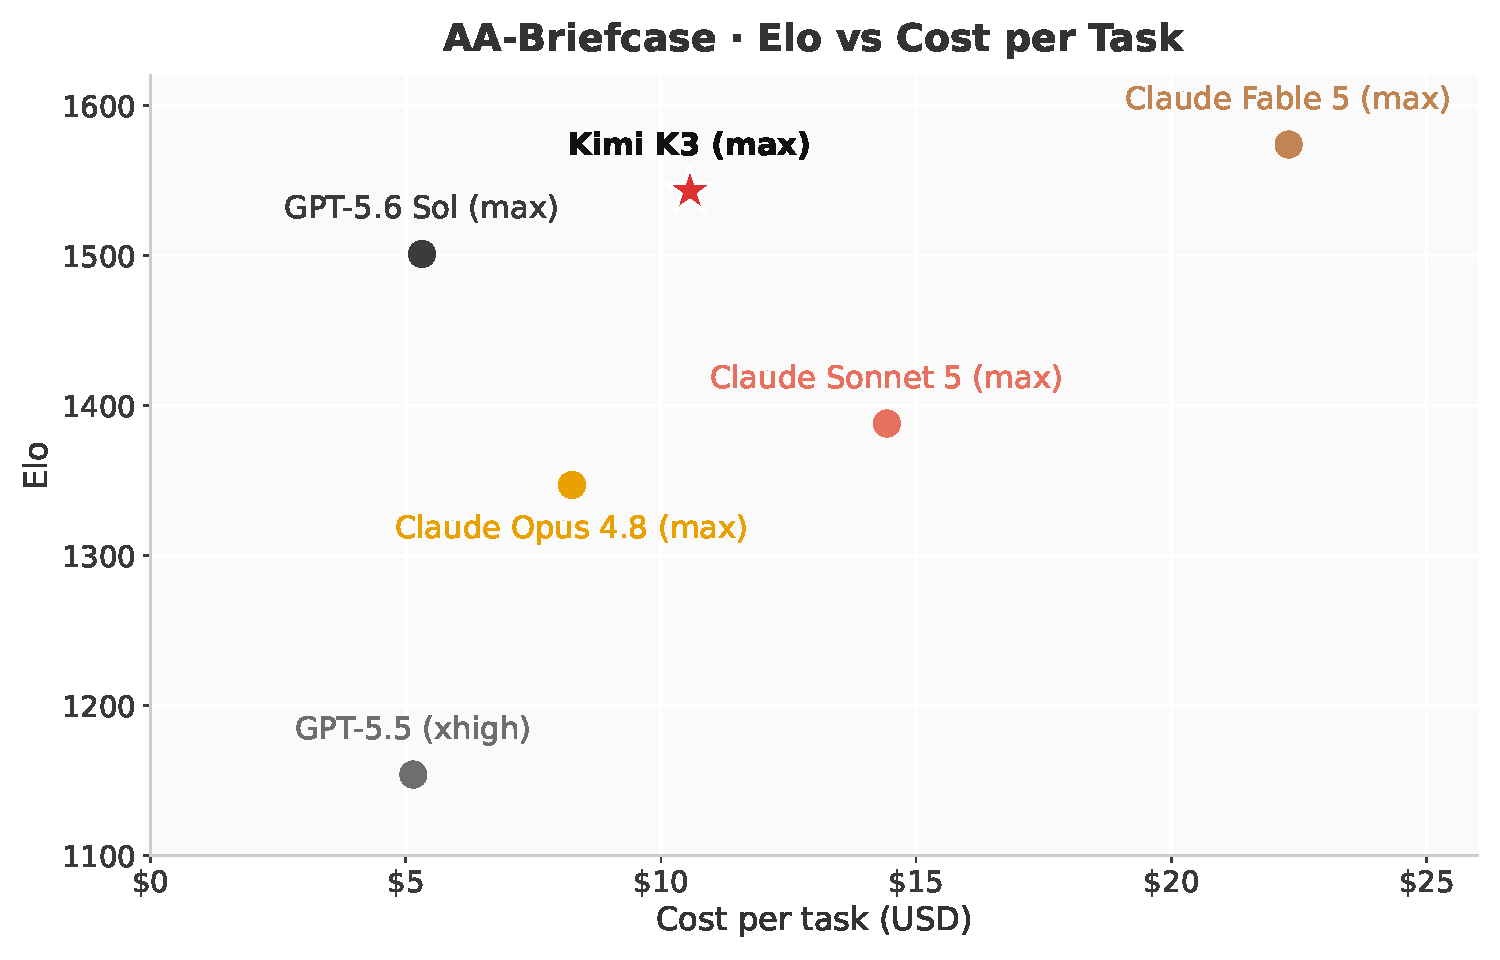
\includegraphics[width=\textwidth]{figures/score_cost_charts/aa_briefcase_score_cost_linear.pdf}\\[2pt]
    {\small (d) AA-Briefcase}
  \end{minipage}
  \caption{Score vs.\ per-task inference cost on Kimi Code Bench~2.0, BrowseComp, GDPval-AA v2, and AA-Briefcase. \kimi{3} is marked with a star.}
  \label{fig:cost_efficiency}
\end{figure}

Overall, \kimi{3} sits on or near the cost-efficiency frontier across all four suites, delivering near-top scores at a fraction of the cost of Claude Fable 5 in particular.
